\documentclass[11pt]{article}
\usepackage{coling2020}
\usepackage{times}
\usepackage{url}
\usepackage{latexsym}
\usepackage{graphicx}
\usepackage{amsmath}
\usepackage{apacite} 
\usepackage{geometry}
 \geometry{
 left=25mm,
 right=25mm,
 top=25mm,
 bottom=25mm
 }
\setlength\titlebox{5cm}

% You can expand the titlebox if you need extra space
% to show all the authors. Please do not make the titlebox
% smaller than 5cm (the original size); we will check this
% in the camera-ready version and ask you to change it back.

% Abstract
\title{Editorial Classification - Bloomberg\vspace{1em}}

\author{
  Aastha Joshi\\
  \texttt{aj2839@columbia.edu}\\
  Columbia University
  \\\And
  Ameya Karnad\\
  \texttt{ak4251@columbia.edu}\\
  Columbia University
  \\\And
  Nirali Shah\\
  \texttt{nss2173@columbia.edu}\\
  Columbia University
  \\\AND
  Sarang Gupta\\
  \texttt{sg3637@columbia.edu}\\
  Columbia University
  \\\And
  Ujjwal Peshin\\
  \texttt{up2138@columbia.edu}\\
  Columbia University
  \\\And
  Smaranda Muresan\\
%   \texttt{Research Scientist}\\
  \texttt{sm761@columbia.edu}\\
  Columbia University
  \\\AND
  Daniel Preotiuc-Pietro\\
%   \texttt{Sr.Research Scientist}\\
  \texttt{dpreotiucpie@bloomberg.net}\\
  Bloomberg LP
  \\\And
  Kai-Zhan Lee\\
%   \texttt{Data Scientist}\\
  \texttt{klee989@bloomberg.net}\\
  Bloomberg LP
  \\\vspace{5em}
}
  

\date{December 20, 2019}

\begin{document}

\maketitle
\bigskip\bigskip
\bigskip\bigskip


\begin{abstract}
 With the influx of myriad news in the Bloomberg terminal, distinguishing editorial news articles from regular articles is critical to aid its users in tailoring their news experience and further analyzing the impact of news on global financial markets. In this paper, we propose various \textit{Machine Learning} and \textit{Deep Learning} models to develop an editorial classifier that generalizes well across various news sources. The training set is made up of articles published by news sources from the US. We compare the performance of these models using the \textit{Macro-Average F1-score} and \textit{Matthews Correlation Coefficient (MCC)} as evaluation metrics to account for the presence of class imbalance in our data. Further, we gauged our models by comparing their performance on a Zero-Shot dataset which comprised of 1805 news articles published by \textit{Metro Winnipeg}, a Canadian news source. 
\end{abstract}

\medskip


\section{Introduction}
\label{sec:intro}

Hundreds of thousands of news stories are published daily across the world. Bloomberg Terminal connects market participants to groundbreaking data through analytics and information-delivery service. This service is used by portfolio managers, investors, analysts, etc. to make investment decisions. The news stories are aggregated from multiple news sources around the globe. A significant portion of these news stories is subjective editorial and opinion content written by staffers or individual contributors with the goal of providing a personal viewpoint, insight or persuading the readers on a certain issue. Editorials shape the public discussion and offer commentary about the important events and issues of the time. They are written by regular columnists (editorials) and by external collaborators (op-eds) in an effort for most newspapers to diversify their opinions and offer a wider, more-specialized discussion on issues. Regular reports are filed by ground reporters and focus on precise factual details describing real-life incidents. 

In contrast with factual news stories, editorials, op-eds, and commentaries are written with the goal of providing the reader with a subjective opinion or commentary, usually backed up by facts. Identifying these stories is useful for faceting and improving search and discoverability. It helps news consumers who are focused on a specific category to access articles pertaining to their interests.

Automatically studying the content of editorials and op-eds has applications in both computer science and social science. First, with the increase in online consumption of news through various channels such as social media. One form of online misinformation can be proliferated by presenting an opinion article as a factual article, lending the credibility of the source to the content. Another application is monitoring of the news or social media stream for potentially breaking news, and opinion articles should be discarded. It is thus paramount to be able to quickly and automatically detect stories from news sources that contain editorial and opinion content. For social science applications, changes in topics or emotional tone with time offer a new lens/perspective in content. Classification of news articles into various categories like regular, editorial, guest, op-ed, etc based on their content before they make their way into the Bloomberg terminal is quite relevant. The information that is streamlined from the Bloomberg Terminal is used to make investment decisions. Having prior information about the category of an article is an important decision marker for the news consumer. This information can also be used by news publication houses to analyze the information being focused on currently and also to develop secondary product features like news recommendation for their product consumers. This information can also be used by researchers who aim to analyze patterns and trends in editorial content. The writing style and vocabulary used by authors of specific categories can provide useful insights to researchers too. 

Several publications provide prospective op-ed with style guides on how to craft their stories. Hence, both due to the subjective and persuasive goal of the editorials and to their different styles, it is feasible to be able to use \textbf{N}atural \textbf{L}anguage \textbf{P}rocessing \textbf{(NLP)} and Machine Learning to automatically identify editorials from factual news stories. NLP offers powerful techniques for automatically classifying documents. These techniques are predicated on the hypothesis that documents in different categories distinguish themselves by features of the natural language contained in each document \cite{ramdass2009document}. Most salient features for document classification may include word structure, word frequency, and natural language structure in each document. The document structure plays an important role in ascertaining the category to which an article belongs to. We aim to use \textbf{NLP} based techniques to process the data from news articles and develop machine learning and deep learning models to classify it. 

This paper presents the first NLP study of opinion content in newspapers.  We have proposed models that are trained on historical archives of news articles. Most of these news articles were published within the span of 2018 - 2019. We use a corpus of stories identified as editorials through newspaper sections. We first build predictive models of editorials using a wide range of linguistics features computed over different sections of the editorials. We conduct an extensive linguistic analysis uncovering the content and style specific of editorials consistent across a wide variety of news sources. Our primary aim is to build a classifier of editorial and regular articles published across news sources. We use statistical techniques to model qualitative trends in language data. We show that using the content of the article, an F-1 macro score of 0.89 can be achieved using the \textbf{XLNet} model on the test data. Our results show that there are marked differences in textual features like word importance, character importance, and document context. Our findings reveal (Section \ref{sec:results}) that quantifying these semantic metrics helps us identify the various categories to which news articles belong based on their content. We present our future work in Section \ref{sec:future}.



\section{Related Work}
\label{sec:relwork}

Recent studies have focused on analyzing the semantic types of claims and premises in online forums\cite{hidey2017analyzing}.  Many techniques focus on the identification of structural and lexical features that happen to be associated with persuasive arguments. Analysis of document structure and semantic features is helpful in extracting useful information about the text. \citeA{habernal2016argument} use lexical features like verbs, tenses, sentiment scores, etc. and experiment with SVM and bidirectional LSTM to predict arguments scored by annotators as convincing. These methods use contextual references to model the data. They try to predict the convincingness of web arguments in an article pair. There has been research to model the features that explore the characteristics of communication that make someone an opinion leader. 

Machine learning-based approaches are used for the automatic identification of discourse participants who are likely to be influencers in online communication \cite{biran2012detecting} Techniques to measure the variation in the contextuality of language \cite{heylighen2002variation} have also been studied. Nouns, adjectives, articles, and prepositions are more frequent in low-context or formal types of expression; pronouns, adverbs, verbs, and interjections are more frequent in high-context styles. This formed the basis for some of the feature engineering performed for our machine learning models. There has been work done to automatically detect evidence from unstructured text that supported a claim using machine learning-based approaches \cite{rinott2015show}. These techniques use context to detect evidence that can be used to support a claim in the discussion. 

Modeling linguistic patterns has revealed that power differentials between participants are subtly revealed by how much one individual immediately echoes the linguistic style of the person they are responding to \cite{danescu2012echoes} This is relevant for our task as the authors for regular, editorial and other categories might have common subtle language markers across the multiple news sources from which the data has been collected.   



% related work & your contributions

\section{Data}
\label{sec:datacol}

In this section, we talk about the Data and the news text and feature collection. We also mention the different programming packages and tools that were used for this task

\subsection{Dataset}

The data was obtained from Bloomberg. The initial data consisted of URL, News Source and Editorial labels. The editorial labels consisted of different categories such as  Regular (regular news), Editorial, Oped, Guest (guest editorial), Roundup (multiple editors), and Others. The data obtained consisted of articles dated from 2008, but most of the articles were as recent as 2018 and 2019. The data consisted of news articles from 95 English news websites. 

\subsection{News text and features collection} 


As the initial dataset did not consist of the news content, article content had to be retrieved by extracting features from the HTML file of the URL present in the initial dataset. For this purpose, we decided to select a sample of 10 news sources on which initial news article text and feature collection would be performed. As all of the news sources had a high percentage of regular articles (It was noted that "Regular" labeled news items formed about 99.1\% of all labels), it was decided that the data would be collected for the top ten news sources with a high count of minority labels. The news sources were, 


\begin{itemize}
  \setlength\itemsep{-0.25em}
  \item New York Times
  \item Washington Post
  \item Washington Observer Report
  \item Digital Journal
  \item Enid News
  \item Californian
  \item Press Democrat
  \item NW Florida Daily
  \item Gazette-Mail
  \item NJ Spotlight
\end{itemize}

The resultant data set had 35394 Articles. The articles are dated from 2013 onwards, but most of them are from the year 2018 and 2019.
% Discussion of the data set and exploratory data analysis
\section{Exploratory Data Analysis}
\label{sec:eda}

We will explore different features of news articles in our dataset.

\begin{figure}[!htb]
\center{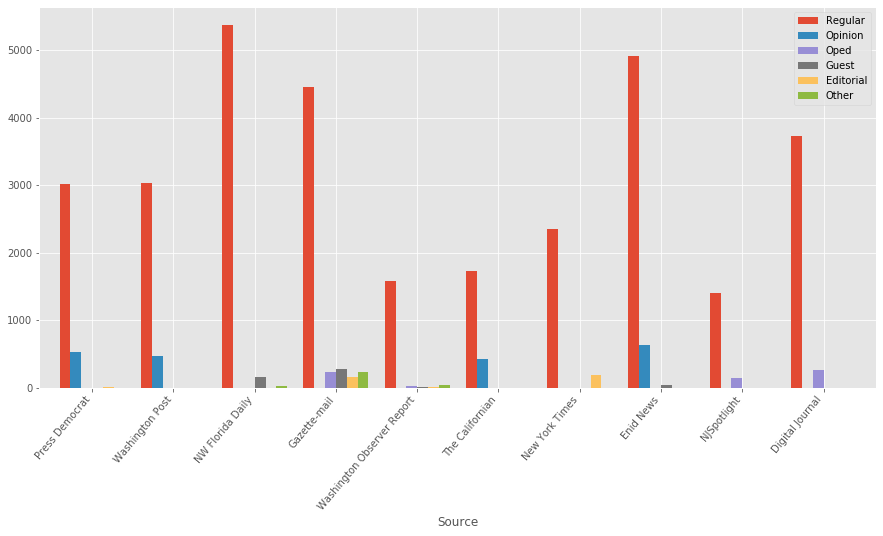
\includegraphics[scale=0.4]
{figures/articles_all_categories.png}}
\caption{\label{fig:d1}  \textit{Distribution of articles per category}}
\end{figure}

\subsection{Categories of Articles}
As mentioned before, the news articles in our dataset were had 6 categories: \textbf{Regular, Opinion, Oped, Editorial, Guest and Other}. To understand the distribution of news articles better, we visualized the \textit{number of news articles} published in these categories across the 10 news sources we have worked on. The result is presented in \textit{Figure \ref{fig:d1}}.

As is evident, most of the articles belong to the \textbf{Regular} category while few articles belong to the rest of the categories. This distribution prompted us to combine the 5 minor categories into a single category called \textbf{Non-Regular}. Another reason why the 5 minor categories were merged is because of the content of these article categories as described in section \ref{sec:intro}. All these categories had articles that were opinionated. Regular category articles are published by ground reporters who reported on stories that are factual. The other categories, \textbf{Opinion, Oped, Editorial, Guest} and \textbf{Other} are all opinions of various people about different events that are based on individual perspectives. Consequently, we will be merging these five labels into the  \textbf{Non-Regular} Class.
Moving forward, we would refer to these 5 categories as part of the \textbf{Non-Regular} class unless otherwise specified. So ultimately, all the news articles would either be in the\textbf{ Regular} class or \textbf{Non-regular} class

We visualized the newly categorized data across the news sources to explain the distribution of articles across the newly developed categories within each news source. The bar plot is presented in \textit{Figure \ref{fig:d2}}.

\begin{figure}[!htb]
\center{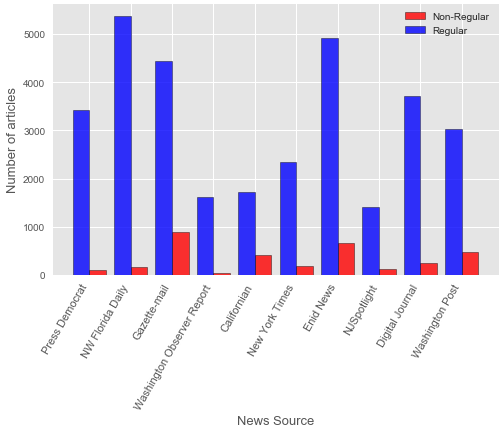
\includegraphics[scale=0.5]
{figures/articles_2_categories.png}}
\caption{\label{fig:d2}  \textit{Distribution of Articles - Regular and Non-Regular}}
\end{figure}

As anticipated, there exists a heavy imbalance in the data with \textbf{Regular} being the major category. To build a model that can accurately classify news articles, it is important to have a balanced dataset to ensure that the model does not predict the majority class by default. This visualization was a key factor for us to confirm that we needed to use techniques like \textit{downsampling} or \textit{upsampling} before developing a model.

\subsection{Count of Words}
 To clean the dataset based on the length of news articles, we developed a visualization to depict the distribution of article length across news sources, the result of which is presented in \textit{Figure \ref{fig:d3}}.
 
 \begin{figure}[!htb]
\center{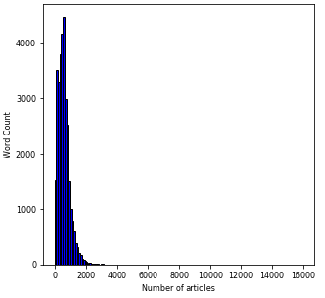
\includegraphics[scale=1.2]
{figures/Word_count_all_sources.png}}
\caption{\label{fig:d3}  \textit{Distribution of Article Length}}
\end{figure}
 
 As seen in \textit{Figure \ref{fig:d3}}, the \textit{95\% confidence interval range for article length} is [100,2000]. Few articles were more than 2000 words long and very few of them had a word count greater than 3000. This derived insight prompted the elimination of articles with word count outside the 95\% confidence interval.
 
  As a part of further inquisition, we analyzed the \textit{word count distribution} of articles for each news source present in our dataset to figure out if the distribution shown in Figure \ref{fig:d3} was heavily impacted by some news sources.
 
 
 We discovered that \textit{The New York Times} generally publishes articles that are up to 4000 words long while most of the articles published by the other news sources are comparatively shorter with a word count of up to 2000.
 This analysis justified that we could clean the dataset based on the word count of articles without losing too much information.
\subsection{Feature analysis}

\noindent
Figure \ref{fig:d4} shows the word cloud generated for news articles belonging to the \textbf{Regular} and \textbf{Non-regular} categories. The entire corpus of training data was used as a document corpus to generate this visualization. In order to extract the words and give them weighting based on their counts, scikit-learn's CountVectorizer was used. The top 50 most common non-stopwords were extracted for each of the 2 categories of news articles.


\begin{figure}[!htb]
\center{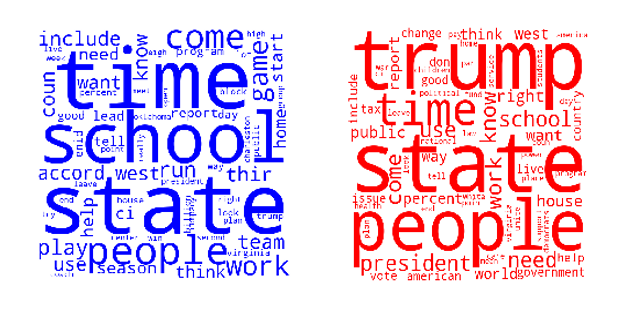
\includegraphics[scale=0.5]
{figures/word_cloud.png}}
\caption{\label{fig:d4}  \textit{Word Cloud - Regular and Non-Regular}}
\end{figure}

\noindent
It can be seen that news articles belonging to the regular category have a common occurrence of words like time, school, state, etc . Whereas for news articles of non-regular category words like trump, president, state, etc. are more commonly used.
This analysis corroborates with the fact that non-regular articles tend to focus more on articles related to politics and current affairs where the author depicts his/her opinion for a given situation. Authors of regular articles are more likely to focus on a variety of topics mostly focusing on the current happening on the ground.

\subsection{Part-of-speech Tagging (POS)}

Part-of-speech (POS) tagging is the process of assigning a word in a corpus as corresponding to a part of speech such as `Nouns', `Pronoun', `Adverb', `Adjective' etc. We explore the presence of different POS tags in the two classes.

To compare the two classes, we first calculate an \textit{Instance per article length} metric for each POS tag which evaluates the percentage of tokens corresponding to those POS tags in the article. We then look at the distribution of \textit{Instance per article length} in the two classes. Our general hypothesis is that the distribution of various POS tags used in \textbf{Regular} and \textbf{Non-Regular} articles would vary. We use the \textit{spaCy} library in \textit {Python} for POS retrieval. The result of our exploratory analysis of POS is presented in \textit{Figure \ref{fig:pos}}. As expected, most of the graphs follow a normal distribution, but there are some striking differences in the distribution of parts of speech in the two classes. Parts of speech like `Adjective' and `Adverbs' seem to be used more frequently used in \textbf{Non-Regular} articles than in \textbf{Regular} articles, perhaps due to the fact that \textbf{Non-regular} articles are more opinionated than \textbf{Regular} articles and provide a more “descriptive analysis” of the `Nouns' (Person/Topic of interest) and `Verbs' (Action of interest), than factual news.  On the other hand, there are more mentions of `Numbers' and `Proper-Nouns' in \textbf{Regular} articles than in \textbf{Non-Regular} Articles. This makes intuitive sense as `Numbers' and `Quantities' convey hard facts.

\medskip
*Note: \textit{The bins in the graphs are left exclusive (i.e the first bin does not include the value 0), So all articles with instance per article length 0 for a particular part of speech will be discarded from the graph. Keys for each of these POS label are present in the Appendix section of the report}

\begin{figure}[!htb]
\center{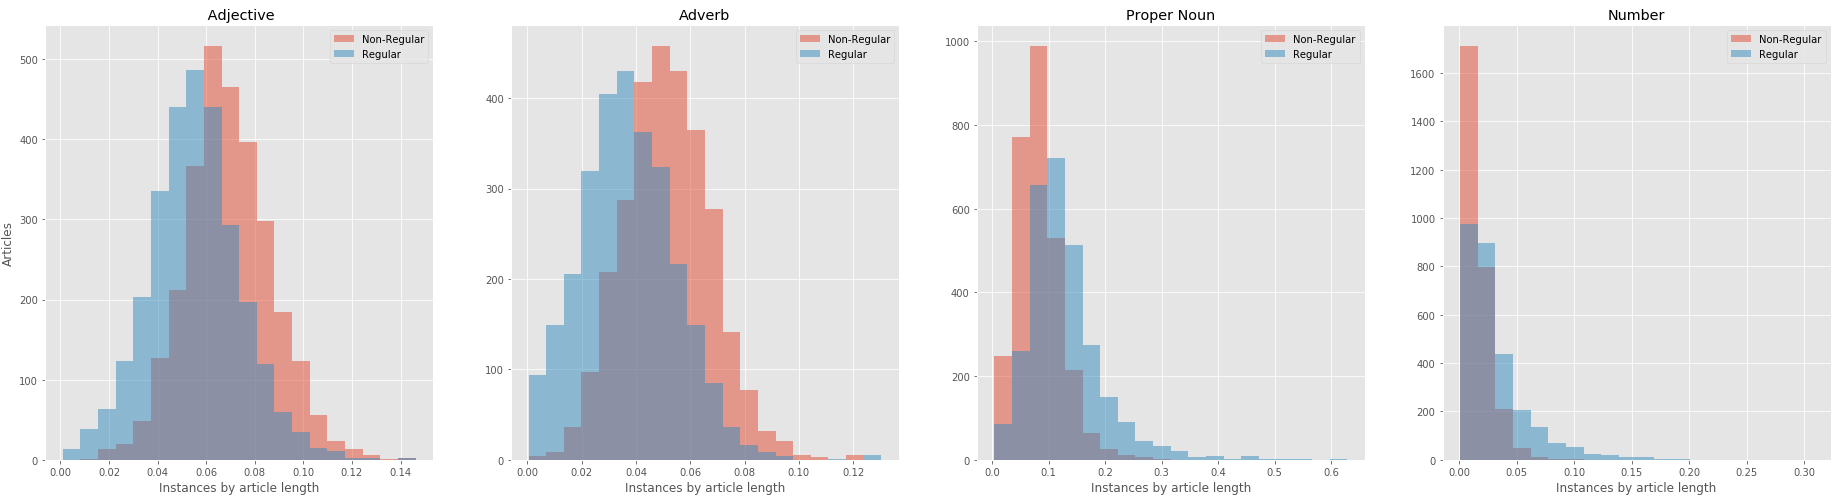
\includegraphics[width=\textwidth]
{figures/pos.png}}
\caption{\label{fig:pos} \textit{Distribution of Parts-of-Speech Tags}}
\end{figure}


\subsection{Named-entity Recognition (NER)}
Named-entity Recognition (NER) aims to recognize mentions of rigid designators from text belonging to predefined semantic types such as `Person', `location', `organization' etc \cite{nadeau2007survey}. Similar to the part-of-speech analysis, we use the NER implementation provided in the \textit{spaCy} package. We calculate the \textit{Instance per article length} for each \textit{named entity} in the two classes.

As can be seen from Figure 2, graphs for Named Entity Recognition were heavily right-skewed for most of the entity types. \textbf{Non-Regular} Articles have  higher mentions of `Law' and `Nationalities' entities as compared to \textbf{Regular} articles in the article text. On the other hand, `Locations', `Product', `Quantity', `Time' and `Date'  have more a prominent presence in \textbf{Regular} articles.

\medskip

*Note :\textit{The Keys for each of these Named Entity Recognition labels are present in the Appendix section of the report}

\begin{figure}[!htb]
\center{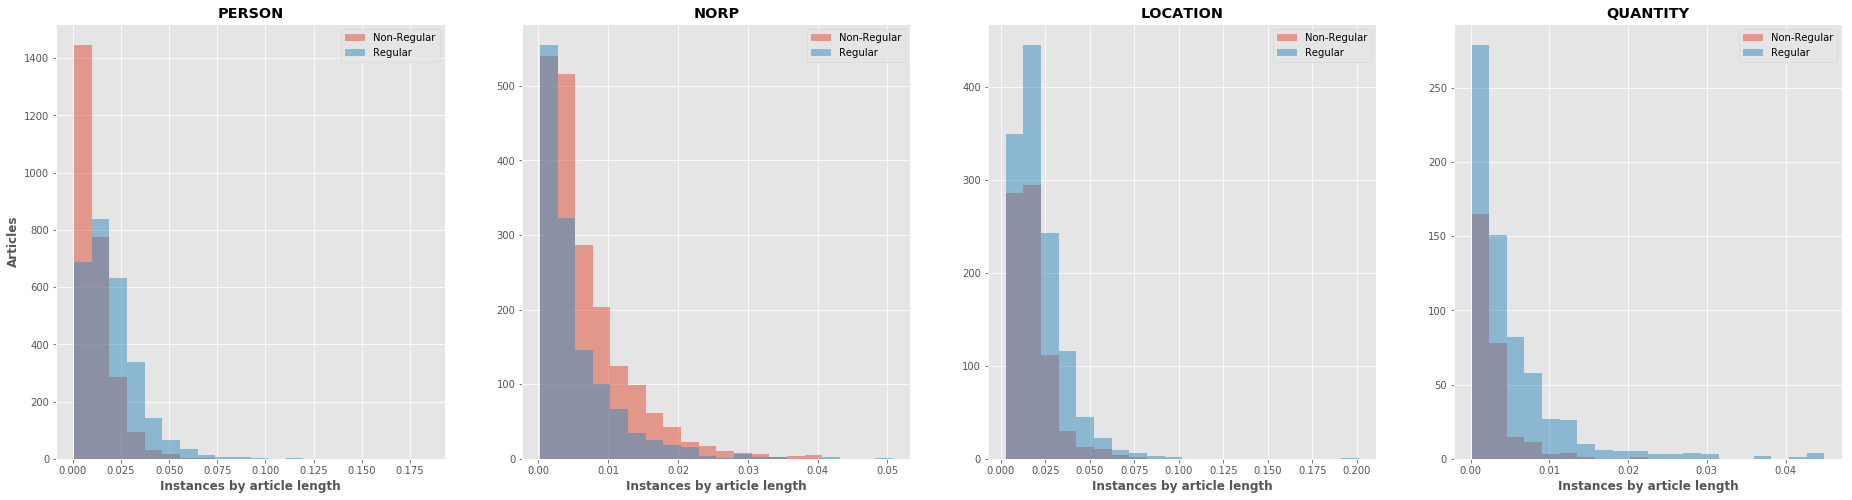
\includegraphics[width=\textwidth]
{figures/ner.png}}
\caption{\label{fig:ner} \textit{Distribution of Named-entity Recognition Tags}}
\end{figure}

\subsection{Correlation Analysis}

Several other features were extracted from both raw articles, processed text (explained in Section \ref{sec:dataprep}), and headlines. General-purpose text features included \textit{average word length} and \textit{sentiment} (using VADER \cite{hutto2014vader}, AFINN \cite{nielsen2011afinn}, and TextBlob) of the article (both retrieved from the processed text). Other features retrieved from the raw articles include \textit{heading length}, \textit{article length}, \textit{number of punctuation} (question marks and exclamations), \textit{subjectivity} (TextBlob).

We conducted a covariance analysis to examine how different features of the articles relate to each other and the target variable. Some significant correlations are visible in the matrix (Insert Figure). For instance, the POS tag for `Proper Nouns' is significantly correlated with `Person' and `Organization' NER tag. This makes sense as person and org names are more likely to be proper nouns than common nouns. There are some significant correlations between article features and the target variable as seen in figure \ref{fig:correlation}(a). Opinion articles, in general, have a higher number of questions  (normalized for article-length) as compared to regular articles (Figure \ref{fig:correlation}(b)). Similarly, regular articles are longer in length than opinion articles. 

\begin{figure}[!htb]
\center{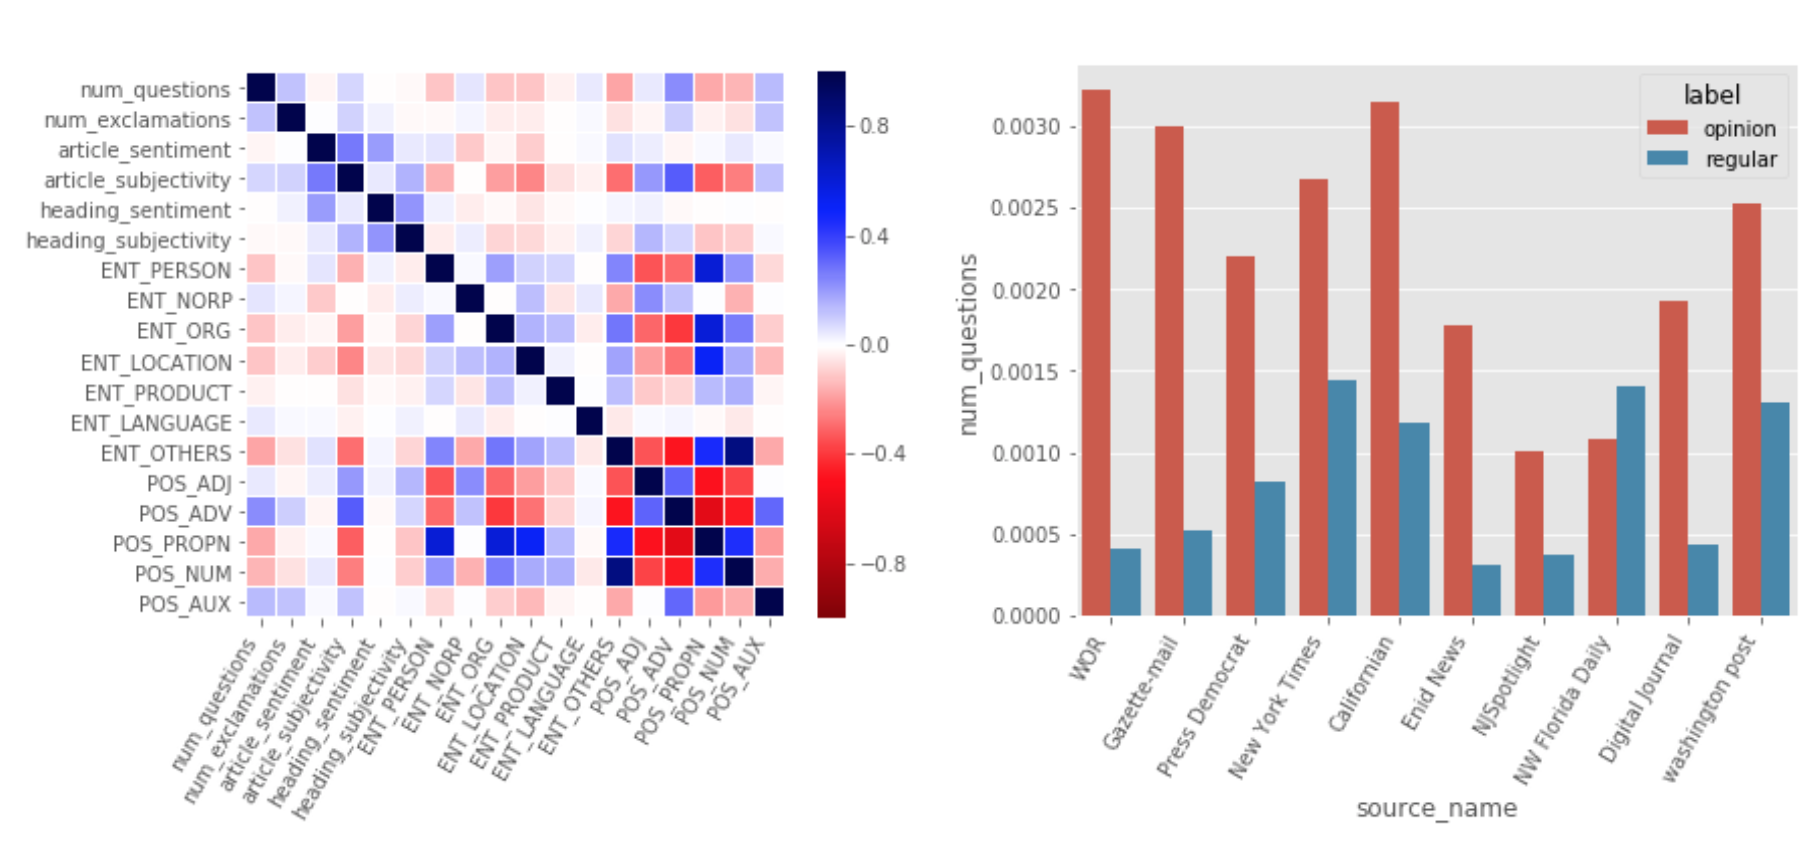
\includegraphics[width=\textwidth]
{figures/feature_correlation.png}}
\caption{\label{fig:correlation} \textit{a) Correlation between features b) Distribution of number of questions by class and source}}
\end{figure}

\section{Data Preparation}
\label{sec:dataprep}
Data preparation is a crucial part of the project. This step works on the data to create features and processed-text that can be used by Machine learning and Deep learning models. The data preparation module used a two-pronged approach to get the data ready:

\subsection{Train-test split and class imbalance handling}
The train-test split are carried out in a temporal fashion. The split it similar to the \textit{TimeSeriesSplit} in scikit-learn where the testing data is in the future of the training data. This was thought of a simulation of a production setting, where a model trained on a few days old data can perform well and does not need to be updated day and again. If we take a 90-10 train-test split, we would calculate a date such that 90\% of the data before it is train and 10\% after it is test. 

After finding that split, another issue is the balance of the dataset. The original dataset has a balance of 89-11 (\textbf{Regular - Non-Regular}). Hence, as mentioned in Section \ref{sec:eda}, we need to undersample the \textbf{Regular} class. We undersampled the data in such a fashion such that, for each instance of \textbf{Non-Regular} class in our dataset, we would have another instance of \textbf{Regular} class from the same news source and from the same date. If there were no articles of \textbf{Regular} class available on the same day, we applied a lookback-lookforward paradigm, where you can pick another article within a lookback and lookward period. As lookforward could lead to potential data leak, we only used lookback of 7 days in our data.

Hence, the training data had 6386 articles (3193 \textbf{Regular} and 3193 \textbf{Non-regular}) and the test set had 3429 articles (3076 \textbf{Regular} and 353 \textbf{ Non-regular})


\subsubsection{Text Processing and Feature Creation}
Additional preprocessed-text was generated, which would aid the generalizability of the model. We took a standard approach to preparing the preprocessed text, which included steps such as, expanding contractions to their full forms using a dictionary of normal contractions, converting to lower-case, removing punctuation, processing HTML, removing URLs from articles, removing stutterings, removing very short words, removing stop words, and Wordnet lemmatization \cite{miller1995wordnet}.

The features were created using both the original text and the preprocessed text. General-purpose text features included Article and Heading lengths, Sentiments (VADER \cite{hutto2014vader}, AFINN \cite{nielsen2011new}, TextBlob), Punctuations (exclamation and question marks), Subjectivity - (TextBlob), Counts of Named Entities and Parts-of-Speech,
Bag-of-words on word-level(unigram, bigram, trigram) character-level(unigram and bigram), TF-IDF on word-level and character-level


\section{Methods}
\label{sec:methods}
\subsection{Logistic Regression}
Logistic regression is a statistical model that in its basic form uses a logistic function to model a binary dependent variable (Regular/ Non-Regular in our project). We developed a \textit{Logistic Regression} model using a count vectorizer as a baseline. Count Vectorizer provides a simple way to both tokenize a collection of news articles and build a vocabulary of known words, but also to encode new articles using that vocabulary. This baseline model was trained on the first 64, 128, 256 ad 512 words.

\medskip
Further, we developed a \textit{Logistic Regression model} using \textit{Term Frequency-Inverse Document Frequency (TF-IDF) Vectorizer} on \textit{unigrams and bigrams} (ngram\_range = (1,2)). TF-IDF is a numerical statistic that is intended to reflect how important a word is to an article in a collection of articles. The TF-IDF value increases proportionally to the number of times a word appears in the article and is offset by the number of articles in the corpus that contain the word, which helps to adjust for the fact that some words appear more frequently in general. The only parameter tuned for this model was \textit{C}.

\medskip
Based on the results shown in \ref{fig:pos} and \ref{fig:ner}, we also trained a Logistic Regression model on the count of different Named Entity 
Recognition and Parts-of-Speech features detected in the news articles. The parameter \textit{C} was tuned to obtain better results.

\subsection{Decision Tree}
One of the standard classifiers we tried was the \textit{Decision Tree Classifier}. A decision tree is a flowchart-like tree structure where an internal node represents a feature(or attribute), the branch represents a decision rule, and each leaf node represents the outcome. It artificially  performs complex decision making. One of the reasons why Decision Tree is so powerful is because it mimics human thinking, thereby making it easily interpretable.

\medskip
We trained a Decision Tree Classifier on TF-IDF vectors generated on unigrams and bigrams from the article text. This model was trained for different sequence lengths viz, 64, 128, 256, 512 and the parameter tuned in each of these individual models was \textit{max\_depth}.

\subsection{Random Forest Classifier}
\textit{Random Forest} is an \textit{ensemble learning} method for classification which operates by constructing a multitude of decision trees on various sub-samples of the dataset and aggregating votes from these trees to decide the final class of the test object. This aggregation limits overfitting, as well as error due to bias and thus, is more robust than a single decision tree.

\medskip

As in case of all the models above, we ran this model using TF-IDF Vectorizer and n\_gram range = (1,2) on the first 64, 128, 256 and 512 words of the article. To obtain better results, we tuned the parameters \textit{max\_depth} and \textit{n\_estimators}.


\subsection{LightGBM}

Along with other standard classifiers, we also tried LightGBM \cite{ke2017lightgbm}. It is frequently used in Kaggle competitions, trains fast and gives comparable performance to other ensemble models. It is a model that is primarily based on decision trees. It splits the trees leaf-wise instead of tree-depth wise or level-wise. Hence, it leads to faster training time and more reduction in loss \cite{al2019comparison}.

LightGBM uses Gradient-based One-Side Sampling to find which value to split on, which is faster than a Histogram-based approach for finding splits. So, it keeps all instances with higher gradients, and also randomly samples instances which have a lower gradient. The assumption here is that those samples with lower gradient have a smaller training error, and hence the model is already tuned to those samples. The parameters tuned for LightGBM were max\_depth, num\_leaves, n\_estimators, and learning\_rate.

\subsection{LSTM, BiLSTM and BiLSTM-Attn}

The first neural model is a \textbf{L}ong-\textbf{S}hort \textbf{T}erm \textbf{M}emory \textbf{(LSTM)} network \cite{hochreiter1997long}. Tokens ti in a given article T = {t1, ..., tn} are computed for different article lengths viz. 64, 128, 256 and 512. These tokens are mapped to pre-trained \textbf{G}love \cite{pennington2014glove} embeddings and passed through an LSTM layer. This is then passed through a global MaxPooling layer followed by a Dropout layer. Dropout is used for model regularisation and to prevent overfitting. Finally, a Dense layer with softmax activation function is used to compute a probabilistic output score.

Next, a Bidirectional LSTM \cite{schuster1997bidirectional} layer was used to model temporal dependencies. BiLSTM connects 2 hidden layers of opposite directions to the same output. Outputs from both states are not connected but concatenated at each time step. This helps the model to learn additional context.

On further experimentation with BiLSTM, word-level attention( \cite{yang2016hierarchical} was incorporated. A single vector is computed as a sum of resulting contextualized vector representations ($\sum_{i}aihi $) at every timestep t. This is subsequently passed through the final prediction layer. 

Next, a Multi-Input BiLSTM model was developed. The 2 inputs are article heading and text. Both input sources were trained separately and the resultant vectors were concatenated. Subsequently, the final vector was used to predict the class probabilities.

\subsection{BERT}

\textbf{B}idirectional \textbf{E}ncoder \textbf{R}epresentations from \textbf{T}ransformers (BERT) is a deep language understanding model based on transformer networks \cite{vaswani2017attention} pre-trained on large corpora \cite{devlin2018bert} released by Google AI in 2018. The model makes use of multiple multi-head attention layers to learn bidirectional embeddings for input tokens. It is trained for masked language modeling, where a fraction (15\%) of the input tokens in a given sequence are masked and the task is to predict the masked word given its context. BERT uses wordpieces which are passed through an embedding layer and get summed together with positional and segment embeddings. The former introduces positional information to the attention layers, while the latter contains information about the location of a segment. 

Similar to the previous model, we run all 4 different BERT models (BERT base-cased, BERT base-uncased, BERT large-cased, BERT large-uncased) on sequences of lengths 64, 128, 256 and 512. Hugging Face’s BERT implementation \cite{wolf2019transformers} in PyTorch was used.

\subsection{XLNet}
XLNet \cite{yang2019xlnet} is a model that was released by CMU and Google Brain in conjunction in June 2019. It claimed to outperform BERT, which was the previous state-of-the-art in 20 language modeling tasks. 

XLNet is a generalized Autoregressive model, that uses either forward or backward context in order to train the model. XLNet allowed Autoregressive models to learn from forward as well as backward context at the same time. XLNet defined a new training objective called Permutation Language Modelling, which was based on permutations. During training, sentence words are permuted and the model predicts a word given the shuffled context. Similar to BERT, XLNet was trained on base-uncased, base-cased, large-uncased, and large-cased, on sequences of lengths 64, 128, 256, and 512, where the only limitation was that the XLNet large models could not be trained on length 512 due to computation limitations.

% Modeling approaches and a critical discussion of your results

\section{Results}
\label{sec:results}
In this section, we evaluate the models based on certain metrics and discuss some salient findings from the models. We discuss the metrics that we have used to evaluate the models as well as some of the interesting results that we obtained from model runs.

\subsection{Evaluation Metrics}
A complete list of evaluation metrics that were used to establish a comparison between the models are listed in the Appendix. Below, we discuss two of the metrics that enable us to take class imbalance into consideration while evaluating the models.

\subsubsection{Matthews Correlations Coefficient (MCC)}

Introduced by \citeA{matthews1975comparison}, the \textit{Matthews Correlation Coefficient} takes all the four quantities of a 2x2 confusion matrix into account while calculating the metric (as compared to \textit{precision} and \textit{recall}). This lends the metric particularly useful when evaluating the performance of model trained on imbalanced classes. It can be calculated as follows:

$$
\begin{aligned}
MCC  = \frac{TP \times TN - FP \times FN}{\sqrt{(TP + FP)\times(TP + FN)\times(TN + FP)\times(TN + FN)}}
\end{aligned}
$$

\medskip

\subsubsection{Macro-Average F-1 Score}

Similar to MCC, the \textit{Macro-Average F-1 score} is a useful metric when the class is highly imbalanced. \textit{Precision} and \textit{Recall} is computed independently for each class and averaged out before calculating the \textit{F-1 score}. Both classes are given equal weights, as is the case in our classification task. The quantities can be calculated as follows:

$$
\begin{aligned}
F1(Macro)  = 2\times\frac{Precision(Macro) \times Recall(Macro)}{Precision(Macro) + Recall(Macro) }
\end{aligned}
$$
$$
\begin{aligned}
Precision(Macro)  = \frac{(\frac{TP}{TP + FP})+ (\frac{TN}{TN + FN})}{2}
\end{aligned}
$$
$$
\begin{aligned}
Recall(Macro)  = \frac{(\frac{TP}{TP + FN})+ (\frac{TN}{TN + FP})}{2}
\end{aligned}
$$

\subsection{Prediction Results}
\textit{Figure \ref{fig:results}} shows the performance of different models on the aforementioned metrics. Performance on the best hyperparameter setting for sequence lengths 64, 128, 256 and 512 are plotted for each model.

For the sake of reporting, the best models out of different types of models were selected. The best model among the LSTM models was the BiLSTM model. The BERT base-uncased model performed the best among all the BERT models. The BERT Large models provided promising results for small sequence lengths, but could not run for larger sequence lengths. Meanwhile, XLNET base-cased worked the best among XLNET models. Similar to BERT Large models, XLNET large models could not run for high sequence lengths.

The reported graphs show that most models perform better at higher sequence lengths. Linear models could run for higher sequences but we decided to restrict at 512 sequence length for the scope of this project as deep Learning models failed to run for higher sequence lengths due to lack of computation resources. 

We found out that XLNet is the best performing model on both the Macro Average F-1 Score metric (Figure \ref{fig:results} (a)) and Matthew’s Correlation Coefficient metric (Figure \ref{fig:results} (b)) followed by BERT. This is most likely due to the fact that XLNet and BERT are pre-trained on a large corpus of English text, which enables it to understand the semantics of the language. Moreover, they have complex architectures that enable them to learn the underlying structure of the data as compared to the linear models. All the other models, on the other hand, have been trained from scratch and do not
provide the benefits associated with transfer learning.

Furthermore, Logistic Regression models fitted with count vectorizer (baseline) and Tf-IDF vectorizer performed better than the three tree-based models.

\begin{figure}[!htb]
\center{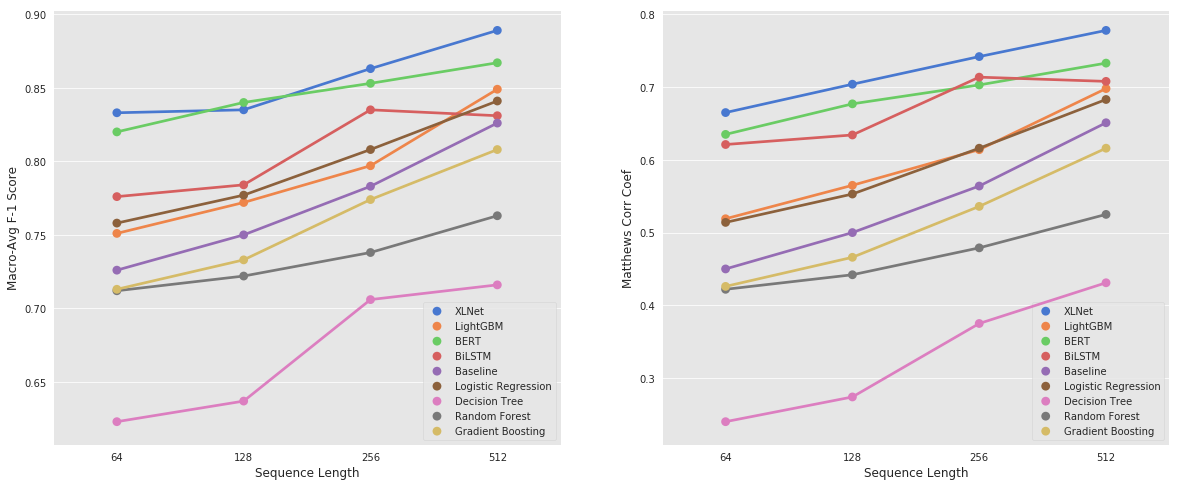
\includegraphics[width=\textwidth]
{figures/results.png}}
\caption{\label{fig:results}  \textit{(a) Performance of different models with their Macro Avg F1 Scores. (b) Performance of different models with their Matthews Corelation Coefficients.}}
\end{figure}



\noindent The comprehensive results can be found on the github link:

\noindent \url{https://github.com/ujjwal95/bloomberg_editorial_classifier/tree/master/etc/results}
\medskip


\subsection{Evaluation on External Data}
The training and test data originated from the same 10 new sources. In order to evaluate the generalizability of our model, we ran the best configurations of each of the models on a zero-shot dataset. Articles from the Canadian Newspaper \textit{The Metro Winnipeg Free Press} was chosen as the zero-shot dataset. This News Source was specifically selected as it a non-US based news source and would allow us to test if the models are generalizable to texts with lexical and topical differences (such as people, locations) with our training data.

The number of articles in the zero-shot dataset were 1805 (1657 \textbf{Regular} and 148 \textbf{Non-regular})
\begin{figure}[!htb]
\center{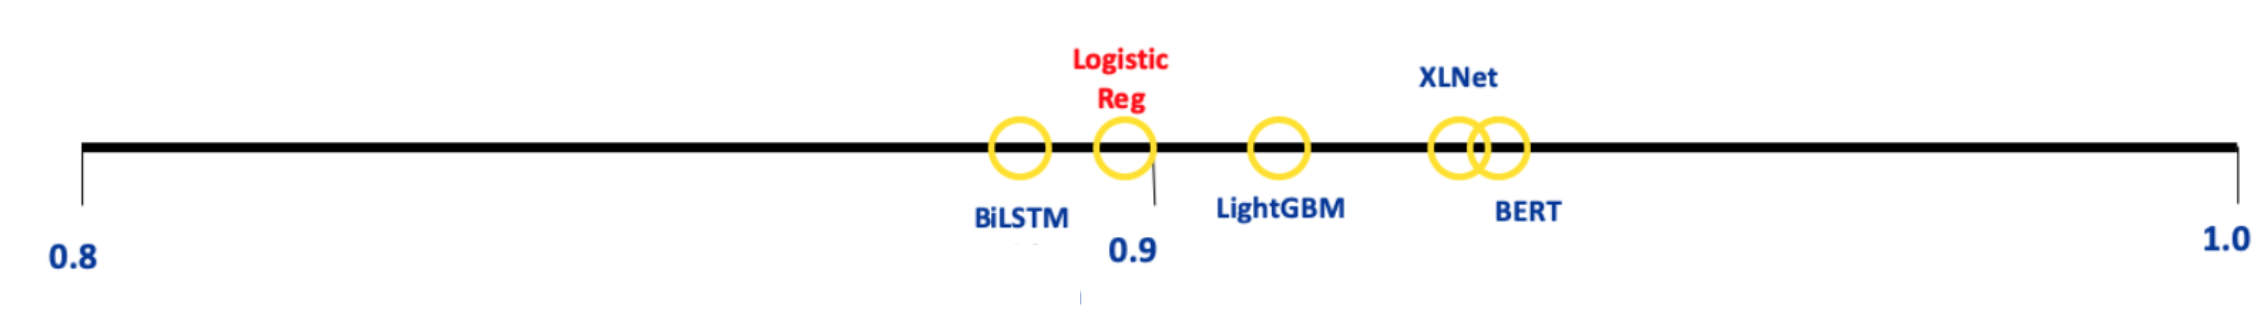
\includegraphics[width=\textwidth]
{figures/f1.png}}
\caption{\label{fig:f1}  \textit{Macro-Average F-1 Score}}
\end{figure}

\begin{figure}[!htb]
\center{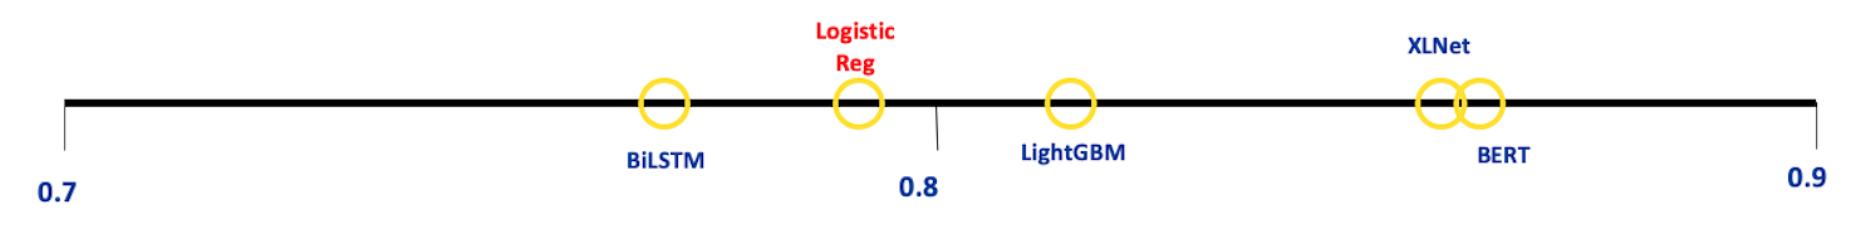
\includegraphics[width=\textwidth]
{figures/mcc.png}}
\caption{\label{fig:mcc}  \textit{Matthew's Correlation Coefficient}}
\end{figure}

As it can be seen from \textit{Figure \ref{fig:f1}} and \textit{Figure \ref{fig:mcc}}, the MCC and Macro-Average F-1 scores are fairly representative of the results obtained on the original validation data. BERT performs the best on the two metrics followed by XLNet. Machine learning models such as Logistic Regression and LightGBM have similar performance to on the validation and the external set. These results imply that the models can be used in a general setting to classify English new articles regardless of their origin.




\subsection{Other Results and Interpretations}


\subsubsection{Feature Importance - Linear Models}

The feature importances generated by the linear model (Figure \ref{fig:fi}) helps us determine the most important features for this classification task. While the most important features varied across different models, the most persistent ones included ‘ENT\_OTHERS’ (Other entities), POS\_PROPN (Proper nouns), POS\_ADV (Adverbs), NEU\_VADER (Sentiment). Specific words like ‘said’ and other characters identified by the TF-IDF vectorizer also had high feature importance.

\begin{figure}[!htb]
\center{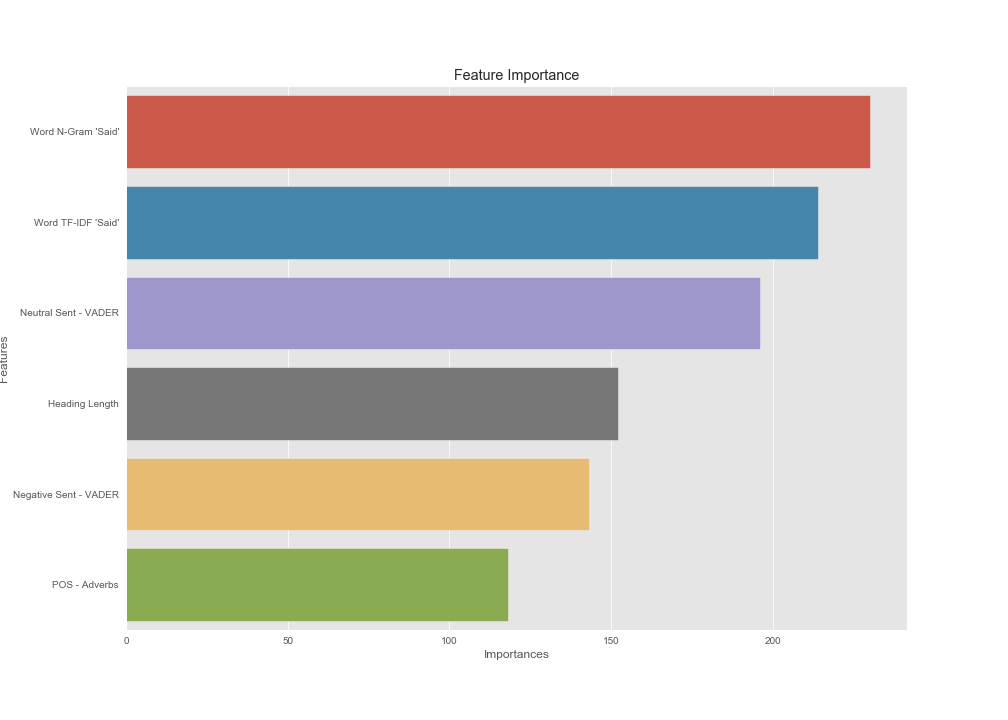
\includegraphics[scale=0.3]
{figures/fi.png}}
\caption{\label{fig:fi}  \textit{Feature importance as per Logistic Regression Model}}
\end{figure}

\subsubsection{Attention in BiLSTM}
Adding attention to our BiLSTM model did show a marginal macro F1 score improvement for word length 128 and 256. However, a slight decrease in the Macro Average F1 score was observed for the word length of 64 and 512. The visualization for the attention for an opinion article with article length as 256 and 64 hidden units of the BiLSTM model is as in \textit{Figure \ref{fig:attention}}.

\begin{figure}[!htb]
\center{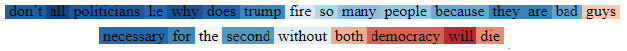
\includegraphics[width=\textwidth]
{figures/attention.png}}
\caption{\label{fig:attention}  \textit{BiLSTM attention based word score}}
\end{figure}


It can be seen from \textit{Figure \ref{fig:attention}} that the model pays more attention to words like why, don't, lie, all, etc. which convey strong emotions of the author. Words like `both', `guys', `democracy', `die', etc. are given a lower score as they are more generic and don't give any strong opinions of the author. 




\section{Conclusion}
\label{sec:con}
Our aim was to build an editorial classifier that can categorize articles from various news sources across the globe as Regular or Non-Regular. To this extent, we evaluated the performance of our machine learning and deep learning models on a Zero-shot dataset which comprised of \textit{1805} news articles published by \textit{Metro Winnipeg}, a \textit{Canadian} news source. This was done to ensure that our models do not categorize articles based on the most frequently occurring topics in articles published by local news sources. While XLNET performed the best on our test data set, closely followed by BERT as can be seen in Figure \ref{fig:results}, BERT outperformed XLNET on the Zero-Shot dataset by a marginal amount. The Macro- Average F1-score was 0.932 for the BERT model and 0.930 for the XLNET model.
An interesting thing to note was that a simple Logistic Regression model with TF-IDF vectorizer and n\_gram range = (1,2) had a macro-average F1-score of 89.6.


The main takeaway from this paper is that for better results, it is advisable to use BERT and XLNET. But in the case of lack of Hardware and computational resources, it is recommended to use Logistic Regression as the model's performance is quite comparable to the deep learning models and unlike deep learning models, it does not lose out on model explainability. Moreover, Logistic regressions are able to incorporate the entire sequence for prediction, which may imporve their performance. Moreover, Logistic Regression models can incorporate the entire sequence for prediction which increases the chance of better prediction as shown in Sections \ref{sec:results}




\section{Future Work}
\label{sec:future}


With the news article data source that is currently available, there is an opportunity to explore more in the domain of News media.

\subsection{Multi-class Classification}

The scope of our project was currently restricted to a binary classification of News articles into Regular and Non-Regular categories. But as future scope of this project, we would be looking to explore the Non-Regular class more and design a multi-class classification system to classify articles into \textbf{Opinion, Oped, Editorial, Guest and Other} classes. As all the Non-Regular class articles are 'opinionated' article, we would like to explore other features that would differentiate between these labels

\subsection{Fine-grained editorial classification}

Currently, our model looks to classify the entire news article. As a future scope of this project, we would like to extend this project to classify the articles on a paragraph and sentence levels. This may help a ground-reporter to ensure that the news article that he/she is publishing is not perceived to be 'opinionated'. This will also help differentiate "Facts" from "Opinions" in any article.

The challenge this task entails is the lack of data in the small parts of the news article. Hence we would have to develop efficient algorithms that can classify text with less amount of data


\subsection{Topic Modeling}

It would be useful to discover hidden semantic structures in article content using Topic Modeling. Developing a topic model can aid us in extracting abstract topics from a collection of articles. To perform topic modeling, we can use Latent Dirichlet Allocation (LDA) \cite{blei2002latent}. LDA is based on the assumption that each document (news article) in a corpus is a combination of topics inferred across all the documents. The topic structure is unknown, and it observes documents and their content and uses it to infer the topic structure\cite{jacobi2016quantitative}. Using this technique, we can figure out if some news sources and authors tend to publish articles based on a certain set of topics. This can also help us to figure out the most common topics as well as the most frequently used words within the topic. 

A time dimension extension of LDA can also be used to see how keywords in the same topic changed over time. Dynamic topic models \cite{blei2006dynamic} can be used to analyze the evolution of latent topics of a collection of documents over time. This can help us determine the most important talking points and keywords during a particular period of time. 

\subsection{News Sentiment Analysis}

It would be interesting to perform sentiment analysis or opinion mining to determine the sentiment of the news article. Sentiment analysis would also be able to determine the emotional state of the writer. Currently, VADER (Valence Aware Dictionary and sEntiment Reasoner) \cite{hutto2014vader}, which is a part of the Natural Language Toolkit (NLTK) is a rule-based sentiment analysis tool that can help detect if the text has a positive, negative or neutral sentiment. An enhancement of this model can be built by manually tagging different articles with various sentiments and emotions using Amazon Mechanical Turk. Supervised Machine learning and Deep learning models can then be used to help classify the data with a multi-label classification algorithm. This can also be used to model how different news sources frame their content for maximum readership impact.

\subsection{Political Bias and Fake News Detection}

The rise in the accessibility of the internet and the boom of social media has made content creation simple \cite{baly2018predicting}. This has made it easier for everybody to share and spread information online. While this has helped crowdsource journalism and has bought important local news to the foreground, it has left the public unprotected against fake news and misinformation campaigns. Fake news has now meddled with a US Presidential election \cite{allcott2017social}, lead to mob lynchings in India \cite{arun2019whatsapp, bali2019fake}, affected stock market \cite{gingerich_2019} and cause diplomatic incidents \cite{aljazeera_2018, filho_2018}.

Hence there is an need to build supervised machine learning models to identify fake news. Amazon Mechanical Turk can be used to tag real and fake news from given dataset. Later, NLP based Machine learning and Deep Learning discussed in section \ref{sec:intro} can be used to trained and build models to detect fake news.

Similarly, political bias and partisanship in media has also increased in the past few years. Editors of different News media houses are looking to influence people with their points. Hence political bias in editorial articles can also be detected using NLP, supervised machine learning and deep learning techniques. We could also look at how people from different sides speak on similar issues differently to convince their readers of their point. This editorial article analysis can be done using an approach similar to the one used by \citeA{habernal2016argument}. 

\section*{Acknowledgements}

We would like to express our special thanks of gratitude to our mentors from Bloomberg LP, Daniel Preotiuc-Pietro and Kai-Zhan Lee for the opportunity to work with them. We are thankful to them for their guidance throughout the project, and for patiently answering our queries no matter how small they were. We would also like to convey our gratitude to our faculty supervisor, Prof. Smaranda Muresan, whose expert advice on Natural Language Processing helped us throughout the project. 

Lastly, we would like to thank the Data Science Institute, Capstone Project DSI facilitator Prof. Eleni Drinea, and Capstone Instructors Professors Sining Chen and Adam Kelleher for providing us an opportunity to work in an exciting project with these wonderful mentors. 

\bibliographystyle{apacite} 
\bibliography{projectbibliography}

\newpage


\section*{Appendix}

\subsection* {Part of Speech Keys}

\begin{itemize}
\setlength\itemsep{-0.25em}
\item`ADJ' : Adjective -  word that modifies/describes a noun or noun phrase
\item `ADP' : Adposition - cover term for prepositions and postpositions
\item `ADV' : Adverb - word that modifies/describes a verb
\item`AUX' : Auxiliary verb -  verb that adds functional or grammatical meaning to the sentence
\item `CONJ' : Coordinating conjunction - a conjunction placed between words, phrases, clauses, or sentences
\item `DET' : Determiner - word that serves to express the reference of a noun
\item `INTJ' : Interjection - Word or expression that expresses a spontaneous feeling or reaction
\item `NOUN' : Noun -  word that functions as the name of some specific thing or set of things
\item `NUM' : Numeral - Numbers and figures 
\item `PART' : Particle - word with traditional meaning
\item `PRON' : Pronoun -  word that substitutes for a noun or noun phrase
\item `PROPN' : Proper noun -  noun that identifies a single entity 
\item `PUNCT' : Punctuation - punctuation marks such as comma, period, parentheses, etc. 
\item `SCONJ' : Subordinating conjunction - a conjunction that introduces a subordinate clause
\item `SYM': symbol - Special Symbols
\item `VERB' : verb - word used to describe an action, state, or occurrence
\end{itemize}

\subsection* {Named Entity Recognition Keys}
\begin{itemize}
\setlength\itemsep{-0.25em}
\item `PERSON':	People, including fictional.
\item `NORP':	Nationalities or religious or political groups.
\item `ORG':	Companies, agencies, institutions, etc.
\item `LOCATION':	mountain ranges, bodies of water, counter, cities, states, 
buildings, airports, highways, bridges, etc.
\item `PRODUCT':	Objects, vehicles, foods, etc. (Not services.)
\item `EVENT':	Named hurricanes, battles, wars, sports events, etc.
\item `WORK\_OF\_ART':	Titles of books, songs, etc.
\item `LAW':	Named documents made into laws.
\item `LANGUAGE':	Any named language.
\item `DATE':	Absolute or relative dates or periods.
\item `TIME':	Times smaller than a day.
\item `PERCENT':	Percentage, including "%".
\item `MONEY':	Monetary values, including unit.
\item `QUANTITY':	Measurements, as of weight or distance.
\item `ORDINAL':	"first", "second", etc.
`CARDINAL':	Numerals that do not fall under another type.
\end{itemize}

\subsection* {List of Evaluation Metrics}

\begin{itemize}
\setlength\itemsep{-0.25em}

\item Precision 
\item Recall 
\item TNR
\item Accuracy
\item Balanced Accuracy
\item F1 Score
\item Matthews correlation coefficient
\item Macro average precision
\item Macro average recall
\item Macro average F1 Score
\item Weighted average precision
\item Weighted average recall
\item Weighted average F1 Score

\end{itemize}

\end{document}
